% !Mode:: "TeX:UTF-8"
%!TEX program  = xelatex

%\documentclass[bwprint]{cumcmthesis}
\documentclass[withoutpreface,bwprint]{cumcmthesis} %去掉封面与编号页

\title{优化汽车后视镜设计}
\tihao{A}
\baominghao{201723003xxx}
\schoolname{电子科技大学}
\membera{卫佳杰}
\memberb{谢沁余}
\memberc{任彦璟}
\supervisor{覃思义}
\yearinput{2017}
\monthinput{07}
\dayinput{13}

\begin{document}
 \maketitle
\begin{abstract}
 
\par 本文建立了双曲率后视镜的最优设计模型,提供了判断后车距离和方位的方法并分析误差,最后用奇瑞QQ的数据代入求解。
\par 本⽂设计的后视镜是由两个不同半径的球面拼接而成,在国家标准两曲率半径相近的要求下,可视为拼接边缘光滑。以左后视镜为例,本文定义水平视野范围为10米外能看到的最大水平宽度,垂直视野范围为后车轮处能看到的最大垂直高度。将原图像抽象为点阵,本文畸变率定义为后视镜成像对应的点阵在消除图像大小变化因素后,所有点两两距离求和的改变程度。本文通过计算机模拟和反射定律求解视野范围和畸变率。单位$1$与畸变率的差值和视野范围相乘得出非畸变的平均视野范围,将该指标作为汽车后视镜设计的优化目标。通过求解得出后视镜曲率半径分别为$1260mm$,$1100mm$,分界线位于距后视镜外侧$\frac{1}{5}$处。
\par 本文通过多项式回归的方法建立后车在凸面镜成像的宽度占主视野区宽度的比例和像距后视镜内边缘的距离与两车前后及水平距离的关系式,得到判断距离的方法,并计算剩余标准差。例如,当像占主视野区的比例为$\frac{1}{2}$且像距后视镜内侧边缘为$2cm$时,两车前后距离为$12m$,左右距离为$2m$,前后距离和左右距离的剩余标准差分别为$4$,$0.5$。
\par 本⽂选⽤奇瑞QQ验证模型,该车型采⽤曲率半径为$1200mm$的后视镜,以左外后视镜为例,得到水平视野范围为$4553mm$,垂直视野范围为$642mm$,畸变率为$2.9\%$。本⽂设计的双曲率后视镜水平视野范围为$5527mm$, 垂直视野范围为$692mm$,畸变率为$3.8\%$;对⽐得出本文设计的后视镜在畸变率基本不变的基础上,视野范围⼤⼤增加,因此优于原设计。

 
\keywords{畸变率  \quad 视野范围  \quad 目标规划 \quad 光学原理 \quad 光学投点}
\end{abstract}

\tableofcontents
\newpage

\section{问题重述}
 

\subsection{引言}

\par 野范围尽可能覆盖汽车的两侧与后方的区域,以便驾驶员能够全面地了解车后方的道路情况。

\par 最常见的是一种双曲率后视镜,内侧接近平面镜,外侧则是一个凸面镜,在它们之间进行了平滑的过渡。为了便于驾驶员对距离进行判断,镜中由虚线或细实线示意了不同曲率的镜面间的分界线(如图(\ref{title})所示)。当然还可以考虑更多曲率以及之间的过渡形式。比如,在侧方位停车时,需要看到后车轮的位置,可能考虑在后视镜下方能有曲率变化。

\begin{figure}[!htb]
\centering
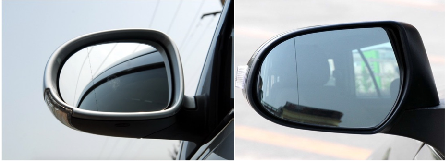
\includegraphics[width=\textwidth]{title.png}
\caption{变曲率后视镜示例}
\label{title}
\end{figure}

\subsection{问题的提出}

围绕优化汽车后视镜的设计、验证过程,本文依次提出如下问题:

\begin{enumerate}
  \item 假设两面外后视镜都设计成双曲率后视镜(或多曲率后视镜),建立相应的数学模型,在后视镜面积一定的条件下,对外后视镜给出优化的设计方案,包括镜面的曲面外形以及分界示意线的位置。
  \item 请就设计的最优后视镜,给出一种方便司机简单易行的快速判断镜中物体的距离与方位的方法。该判别方法要考虑一定的误差。
  \item 以一种现有的轿车为例,镜面的边缘轮廓可以沿用现有的设计的基础上,给出具体的计算结果。 
\end{enumerate}

\section{问题分析}

\par 在国家车辆标准的现有基础上,对左侧后视镜的视野范围定义为驾驶员能看到后视镜后方10米处,距离车身的范围。对右侧后视镜的视野范围定义为驾驶员能看到后视镜后方20米处,距离车身的范围。我们采用畸变率来衡量驾驶员看到的图像与实际图像的偏差。如果汽车的后视镜使用平面镜,图像没有畸变,对距离和方位的判断十分准确。但是当镜面大小受限时,视野相对较小。如果使用凸面镜,可以以较小的镜面获得更加宽广的视野,但是图像存在较大畸变,难以准确判断镜中物体与自己的距离及镜中物体与自己的相对方位。汽车外后视镜的设计需要满足视野尽可能大的同时减少图像的畸变率。

\subsection{问题一}

\par 设计的双曲率外后视镜,首先要确定曲率半径不同下的两球面的球心坐标,通过球心的坐标,确定球面的位置,得到球面方程,通过反射定理,得出双曲率外后视镜的畸变率及左右外后视镜各自的的水平(垂直)视野范围,在畸变率保持在可接受范围内的基础上,使外后视镜的视野范围最大。同时确定出双曲率后视镜两不同曲率的最优分界线。
\subsection{问题二}

\par 在问题一设计的基础上确定驾驶员看到的后方车辆在镜面上的图像的宽度占外后视镜宽度的比例,给出司机简易快速判断后视镜中物体与本车距离、方位的判断方法。收集统计量产车数据得到常见车辆平均宽度数据,经过模型计算得到后视镜中像的大小与后车车距的比例关系,并且分析快速判断方法造成的误差。
\subsection{问题三}

\par 根据选定的量产车的实际数据,计算得到评价模型的各个参数。 

\section{模型的假设}

\begin{enumerate}
	\item 本文设计的双曲率球面外后视镜在分界线两侧保持曲率恒定,忽略过渡处,认为过渡处可用工艺加工变平滑。
	\item 最初按照最小模型($70mm \times 72.48mm$)设计,再对照实际进行等比放大和截取,从而得到最终设计的外后视镜。
	\item 在计算畸变率时,取眼点连线的中点处作为人眼的位置。
	\item 平均车宽取1700mm。  
\end{enumerate}


\section{符号说明}
\begin{table}[!h]
\centering
\begin{tabular}{cc}

\toprule
 \makebox[0.4\textwidth][c]{符号}	&  \makebox[0.5\textwidth][c]{意义} \\ \midrule
 $\alpha$	& 平均畸变率 \\ 
 $K$	    & 综合指标  \\ 
 $L$	    & 水平视野范围  \\ 
 $H$	    & 垂直视野范围  \\ 
 $Q_1$	    & 主视野区(大曲率半径)镜面球心  \\ 
 $Q_2$	    & 副视野区(小曲率半径)镜面球心  \\ 
 $R_1$	    & 主视野区(大曲率半径)曲率半径  \\ 
 $R_2$	    & 副视野区(小曲率半径)曲率半径  \\ 
 $cutRatio$ & 副视野区所占的比例\\
 $dis$	    & 光屏距离外后视镜的距离  \\ 


\bottomrule 
\end{tabular}
\end{table}
\section{模型建立}
\subsection{视野范围模型}

\begin{figure}[!h]
\centering
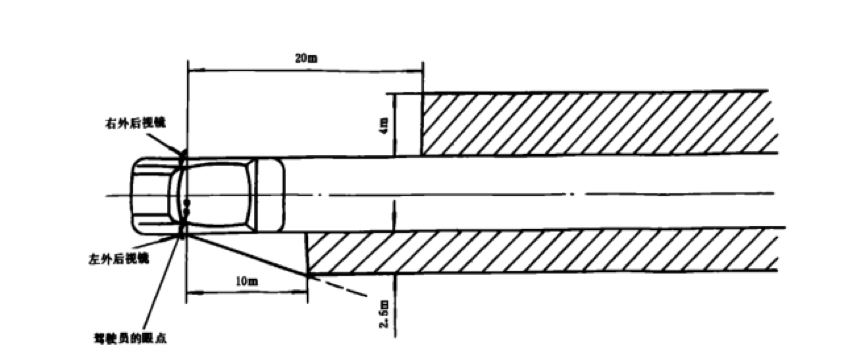
\includegraphics[width=\textwidth]{view.png}
\caption{水平视野范围的定义}
\label{view}
\end{figure}

\par 在司机的最大视野范围模型中,在水平方向上根据国家标准$GB 15084-94$(如图(\ref{view})所示),对左侧后视镜,将距后视镜10米处,司机从后视镜所能观测到的水平宽度定义为左侧的水平视野范围$L$。同时根据国家标准$GB 15084-94$,通过调整后视镜的空间方位,驾驶员借助左侧后视镜必须可观测到水平宽度为2.5米的水平视野区域,将该视野范围定义为左侧水平视野范围下限。
\par 同理,对右侧后视镜,将距后视镜20米处,司机从后视镜能观测到的水平宽度定义为右侧的水平视野范围$L$,右侧水平视野范围下限为4米\upcite{GB}。
\par 如图(\ref{hight})所示,将通过外后视镜在后车轴处能够观测到的垂直视野高度定义为垂直视野范围$H$。

\begin{figure}[!htb]
\centering
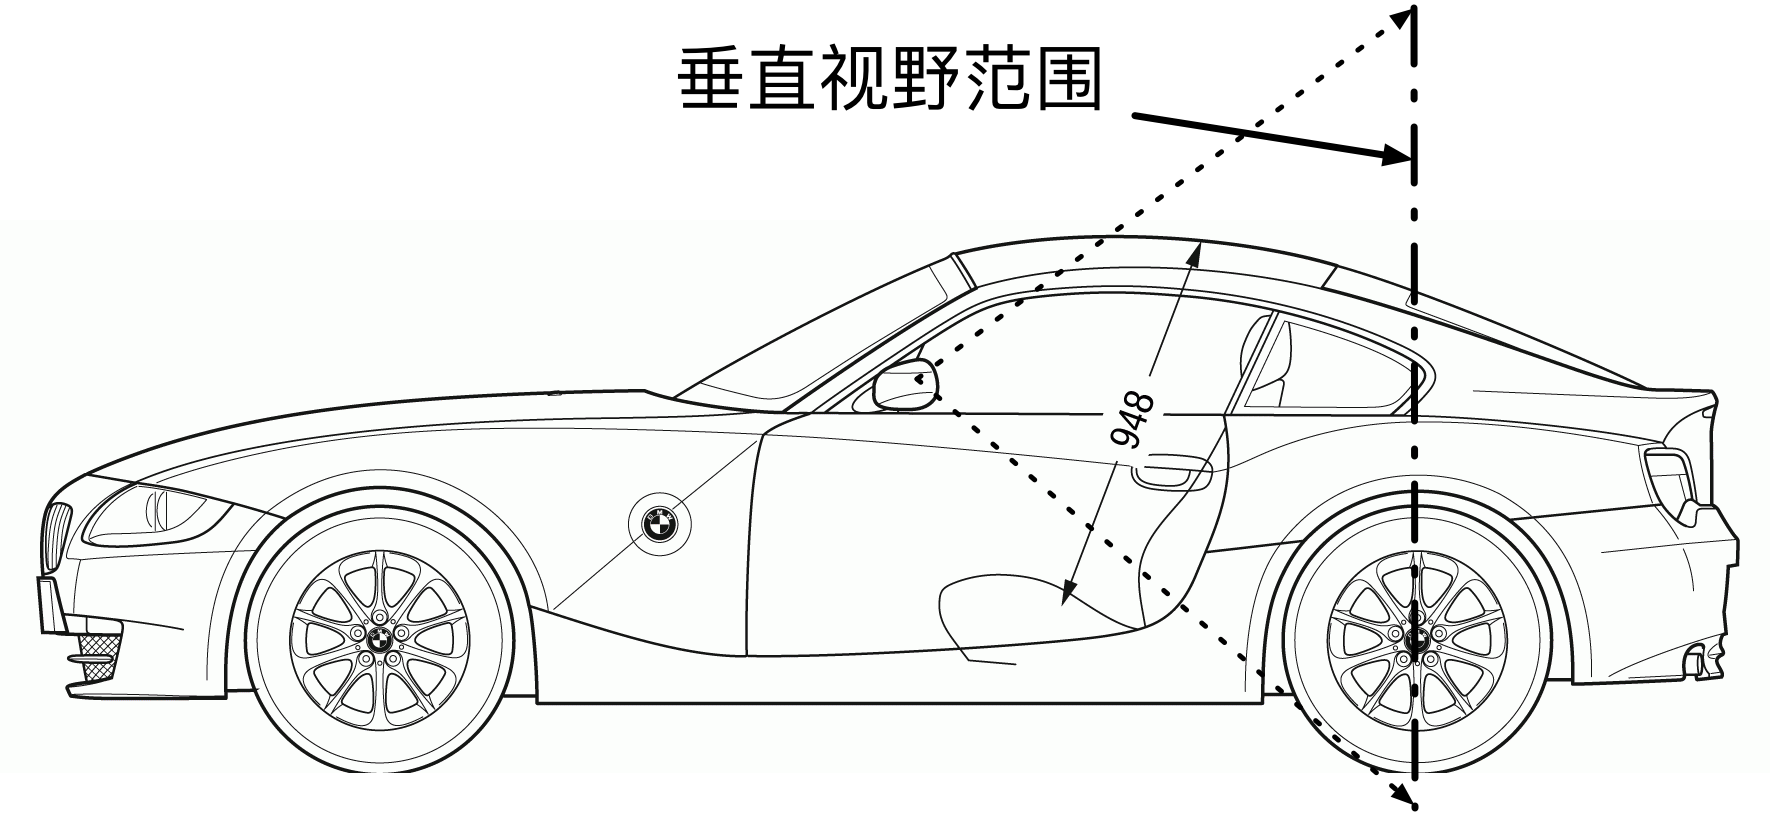
\includegraphics[width=12cm]{hight.png}
\caption{垂直视野范围的定义}
\label{hight}
\end{figure}

\subsection{平均畸变率模型}
\subsubsection{平均畸变率模型的建立}

\par 畸变率是衡量汽车后视镜是否合格的一个重要的技术指标,我们提出平均畸变率衡量指标,以便分析和对照\upcite{大视野后视镜} 。

\par 将镜面放置于$XOZ$平面,并作平行于坐标轴$n \times m$的网络划分,选取各个网格点与眼点的连线,作为入射光线,由反射定律得到反射光线,在平行于$XOZ$平面的面$(y>0)$处设置无限大光屏接收反射光线,得到对应的$n \times m$的网格点。
\par 对镜面上$n \times m$的任意两网格点$(i,j)$对之间的距离$D_{ij}$求和:

\begin{equation}
	\sum\limits_{i = 1}^{n}\sum\limits_{j = i + 1}^{m} D_{ij}
\end{equation} 

\par 对接收光屏上$n \times m$的任意两网格点$(i,j)$对之间的距离$d_{ij}$求和:

\begin{equation}
	\sum\limits_{i = 1}^{n}\sum\limits_{j = i + 1}^{m} d_{ij}
\end{equation}

\par 随着接收光屏与镜面间的距离增大,接收屏上的网格点间距同比增大,但是对于可看到的图像的外形没有影响,因此建立相似比系数来消除图像放大对格点间距离的影响。

\par 我们将相似比定义为镜面上 $n \times m$ 的格点构成的区域最长边长$L_{max}$ 与接收屏上 $n \times m$ 的格点构成的区域最长边长$l_{max}$ 的比值 $\beta$。如图()所示,将矩形区域宽高中较大的值作为其区域最长边的边长。

\begin{equation}
	\beta = \frac{L_{\mathop{max}}}{l_{\mathop{max}}} \times 100 \%
\end{equation}



\begin{figure}[!htbp]  
\begin{minipage}[t]{0.5\textwidth}
\centering  
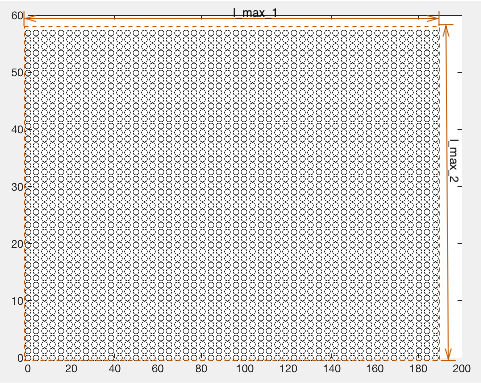
\includegraphics[width=\linewidth]{L1.png} \\
\caption{镜面上投点示意图} \label{L1}
\end{minipage}
\hspace{1ex}
\begin{minipage}[t]{0.5\textwidth}  
\centering  
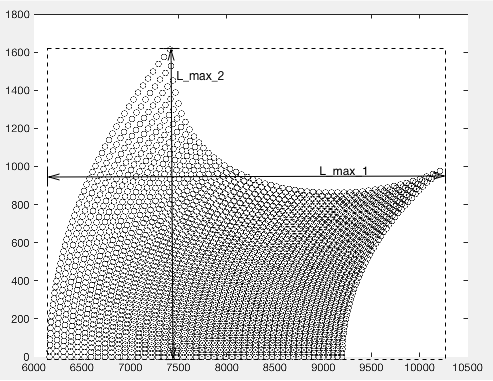
\includegraphics[width=\linewidth]{L2.png}\\
\caption{光屏接收光线落点示意图}  \label{L2}
\end{minipage}  
\end{figure} 


\par 平均畸变率$\alpha$定义如下公式(\ref{畸变率})所示:


\begin{equation}
\label{畸变率}
	\alpha = \frac{\mid \beta \sum\limits_{i = 1}^{n}\sum\limits_{j = i + 1}^{m} d_{ij} - \sum\limits_{i = 1}^{n}\sum\limits_{j = i + 1}^{m} D_{ij} \mid}{\sum\limits_{i = 1}^{n}\sum\limits_{j = i + 1}^{m} D_{ij}} \times 100 \%
\end{equation}


\subsubsection{平均畸变率模型的验证}

\par 按照定义计算得到平面镜的平均畸变率为$4.32402\times 10^{-12}\%$,可以确定在不存在畸变时,模型计算结果约为0。


\subsection{综合评价指标$K$}
\par 建立综合评价指标$K$,描述平均畸变率和视野范围的综合优化结果。计算方法如下公式(\ref{K})所示(其中L表示水平视野宽度):
\begin{equation}
\label{K}
	K = (1 - \alpha) \cdot L
\end{equation}

\subsection{镜面模型}
\subsubsection{镜面模型的球心坐标}

\par 对于镜面模型的建立,考虑外后视镜中线与无限远处地平线重叠,简化球心坐标求解所用的坐标系到二维$XOY$平面上。 确定如下图(\ref{basic})所示的坐标系(由Z轴正半轴向负半轴观察):

\begin{figure}[!htb]
\centering
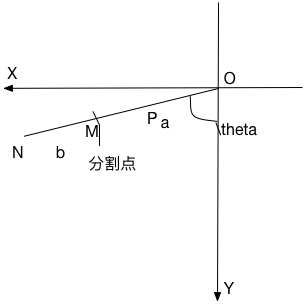
\includegraphics[width=8cm]{basic.png}
\caption{镜面坐标系建立}
\label{basic}
\end{figure}


\subsubsection{镜面模型方案一}

\begin{figure}[!htbp]  
\begin{minipage}[t]{0.5\textwidth}
\centering  
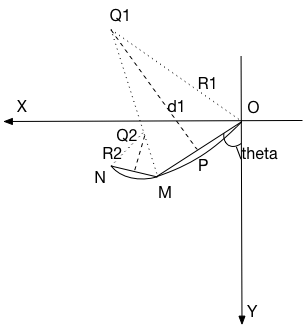
\includegraphics[width=\linewidth]{plan1.png} \\
\caption{方案一镜面设计(坐标)} \label{plan1}
\end{minipage}
\hspace{1ex}
\begin{minipage}[t]{0.5\textwidth}  
\centering  
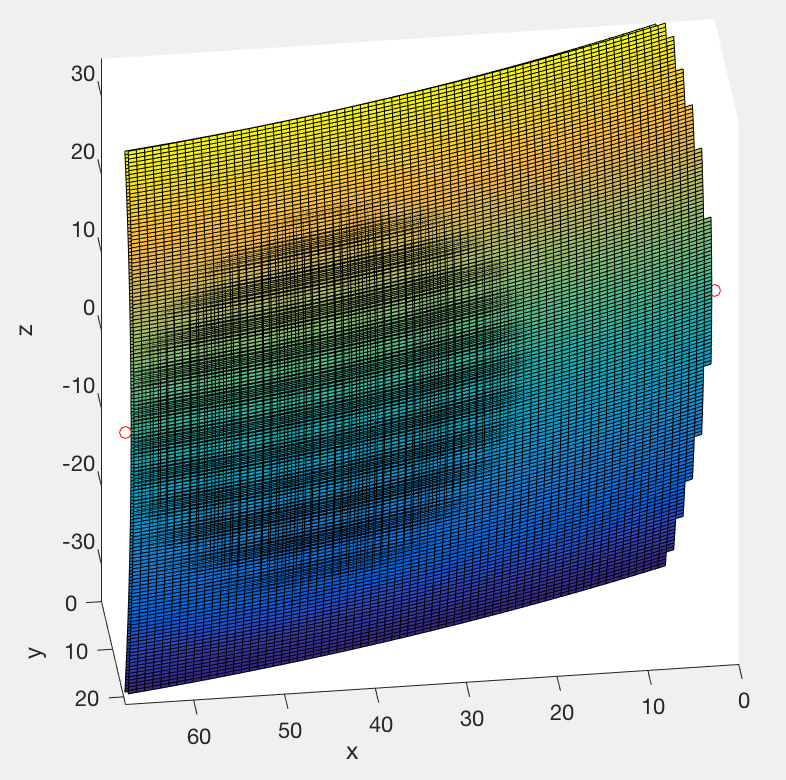
\includegraphics[width=\linewidth]{plan1-0.png}\\
\caption{方案一镜面设计(图像)}  \label{plan1-0}
\end{minipage}  
\end{figure} 


\par 假设左侧外后视镜的水平中线在$XOY$平面内,图(\ref{plan1})为后视镜的在$XOY$平面内的截面。后视镜由两个曲率不同的球面镜组成,两球面在$XOY$平面上的截面的弧线分别为弧$OM$、弧$MN$。

\par 定义$OM = a$, $MN = b$, $a + b = length$, $\frac{b}{a} = cutRatio$,设$Q_1$点的坐标为$(x_1,y_1,0)$,在$XOY$平面上$Q_1$点的坐标为$(x_1,y_1)$ 为镜面截线与$y$轴的夹角。

\par 镜面与$XOY$平面的交线的直线方程可以抽象为公式(\ref{镜面与$XOY$平面的交线的直线方程}):
 
\begin{equation}
\label{镜面与$XOY$平面的交线的直线方程}
	y = \mathop{cot}\theta \cdot x
\end{equation}

$Q_1$点到镜面的距离$d_1$(\ref{d1})即为$Q_1$点到直线$OM$的距离,通过点到直线的距离公式得:

\begin{equation}
\label{d1}
	d_1 = \frac{\mid \mathop{cot}\theta \cdot x_1 + y_1 \mid}{\sqrt{\mathop{cot}^{2} \theta + 1}} 
\end{equation}

\par 对直角三角形$Q_1OP$由勾股定理可得:$ d_1^2 + \left( \frac{a}{2} \right) = R_1^2$,将$d_1$带入得公式(\ref{plan1dis1}):
\begin{equation}
\label{plan1dis1}
	\left( \frac{\mid \mathop{cot}\theta \cdot x_1 + y_1 \mid}{\sqrt{\mathop{cot}^{2} \theta + 1}} \right)^2 +\left( \frac{a}{2} \right) = R_1^2
\end{equation}

\par 由设计可得$P$点坐标为:$P(\frac{a}{2} \mathop{sin} \theta, \frac{a}{2} \mathop{cos} \theta)$

\par 由中垂线定理、$Q_1P$与镜面垂直(即两直线垂直),斜率之积为$-1$得公式(\ref{plan1-1}):

\begin{equation}
\label{plan1-1}
	\frac{y_1 - \frac{a}{2} \mathop{cos} \theta}{x_1 - \frac{a}{2} \mathop{sin} \theta} \cdot \mathop{cot}\theta = -1
\end{equation}

\par (\ref{plan1dis1})(\ref{plan1-1})两式联立可解得:$Q_1(x_1,y_1)$,在空间中大曲率半径镜面的球心坐标为 $Q_1(x_1,y_1,0)$。由设计可知$M$点坐标为$M(a \mathop{sin} \theta, a \mathop{cos} \theta)$,则在二维平面$XOY$内,$Q_1M$的斜率为:

$$k = \frac{y_1 - a \mathop{cos} \theta}{x_1 - a \mathop{sin} \theta}$$
 
\par 可以得到$Q_1M$的直线方程为:
\begin{equation}
\label{plan1-q1m}
	y = \frac{y_1 - a \mathop{cos} \theta}{x_1 - a \mathop{sin} \theta} (x - a \mathop{sin} \theta ) + a \mathop{cos} \theta
\end{equation}

在本设计下,$Q_2$点在直线$Q_1M$上,设$Q_2$点的坐标为$Q_2(x_2, y_2)$,$Q_2$和$M$两点间的距离为小曲律半径镜面的半径$R_2$

\begin{equation}
\label{plan1-r2}
	\sqrt{(x_2 - a \mathop{sin}\theta )^2 + (y_2 - a \mathop{cos}\theta )^2} = R_2
\end{equation}
\par 将坐标代入公式(\ref{plan1-q1m})后与公式(\ref{plan1-r2})联立可解得球心坐标$Q_2(x_2,y_2)$,则在空间中小曲率半径镜面的球心坐标为$Q_2(x_2,y_2,0)$。


\subsubsection{镜面模型方案二}

\par 方案二基于$MNO$三点共线设计,且与方案一使用相同变量名和坐标系,图(\ref{plan2})为后视镜的在$XOY$平面内的截面。


\begin{figure}[!htbp]  
\begin{minipage}[t]{0.5\textwidth}
\centering  
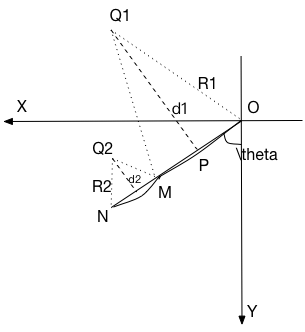
\includegraphics[width=\linewidth]{plan2.png} \\
\caption{方案二镜面设计(坐标)} \label{plan2}
\end{minipage}
\hspace{1ex}
\begin{minipage}[t]{0.5\textwidth}  
\centering  
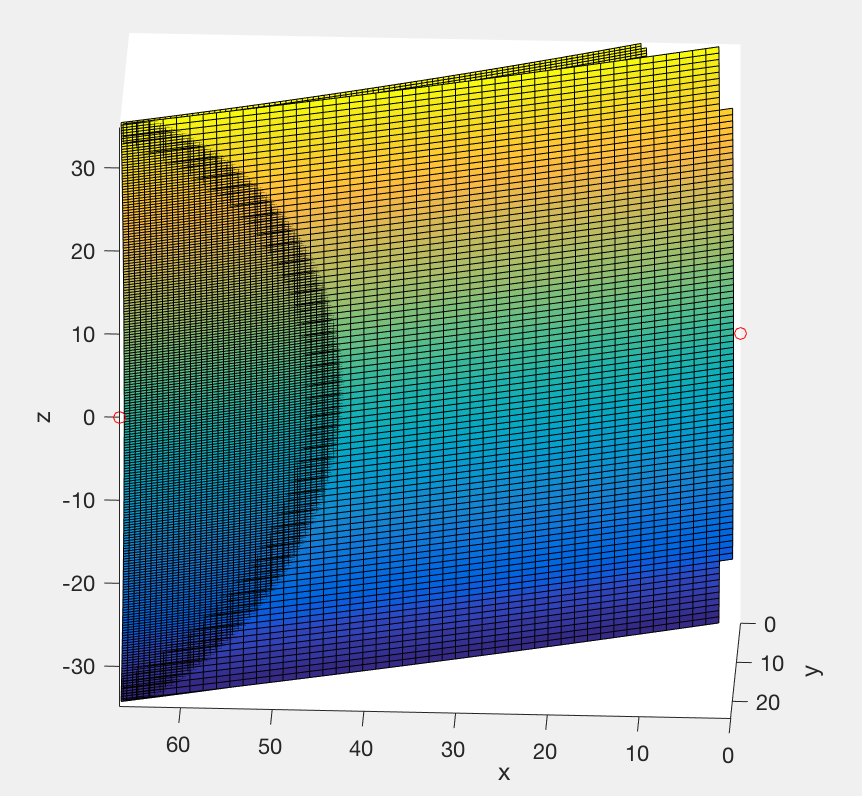
\includegraphics[width=\linewidth]{plan2-0.png}\\
\caption{方案二镜面设计(图像)}  \label{plan2-0}
\end{minipage}  
\end{figure} 

\par 对于大曲率半径镜面的球心$Q_1$的设计与方案一相同,对于小曲率半径镜面的球心$Q_2(x_2,y_2)$,有距离$d_2$:

\begin{equation}
	d_2 = \frac{\mid \mathop{cot}\theta \cdot x_2 + y_2 \mid}{\sqrt{\mathop{cot}^{2} \theta + 1}} 
\end{equation}
\par 对直角三角形$Q_2NM$由勾股定理可得:$d_2^2 + \left( \frac{b}{2} \right) = R_2^2$,将$d_1$代入得公式(\ref{plan2-dis}):

\begin{equation}
\label{plan2-dis}
	\frac{\mid \mathop{cot}\theta \cdot x_2 + y_2 \mid}{\sqrt{\mathop{cot}^{2} \theta + 1}} = \sqrt{R_2^2 - \left( \frac{b}{2} \right)^2} 	
\end{equation}
\par 与方案一同理得公式(\ref{plan2-1}):
\begin{equation}
\label{plan2-1}
	\frac{\left(a + \frac{b}{2}\right) \mathop{cos} \theta - y_2}{\left( a+ \frac{b}{2} \right) \mathop{sin} \theta - x_2} \cdot \mathop{cot}\theta = -1
\end{equation}
\par 联立公式(\ref{plan2-dis})(\ref{plan2-1})解得球心坐标$Q_2(x_2,y_2)$,则在空间中小曲率半径镜面的球心坐标为$Q_2(x_2,y_2,0)$。

\section{模型求解}

\subsection{问题一求解}

\subsubsection{镜面尺寸的确定}
\par $M$类是至少有4个车轮并且用于载客的机动车辆;$M_1$类是包括驾驶员座位在内,座位数不超过9座的载客车。因此本文针对的典型的小型家用轿车属于$M_1$类。根据国家标准$GB 15084-94$中关于后视镜最小尺寸要求标准(如表(\ref{后视镜最小尺寸要求标准})所示)。本文所设计后视镜属于第三类后视镜,且其反射面的曲率半径不得小于$1200mm$。考虑制造公差,反射面曲率半径一般设定在$1260mm$\upcite{后视镜设计} 。

\par 同时根据$GB 15084-94$中4.3.4的规定:镜面上任何一点的曲率半径$r_{pi}$与$r$之差不得大于$0.15r$。

\begin{table}[!htbp]
\centering
\caption{后视镜最小尺寸要求标准}
\label{后视镜最小尺寸要求标准}
\begin{tabular}{cccc}
\toprule
后视镜类别 & 适用汽车类型 & $a$ & $b$	\\ \midrule
 II	 & $M_2$ 、$M_3$ 和$N_2$、 $N_3$ &  $a =  \frac{170}{1+\frac{1000}{r}}$& 200\\ 
III & $M_1$ 和$N_1$& $a =  \frac{130}{1+\frac{1000}{r}}$&  70\\ 
\bottomrule 
\end{tabular}
\end{table}

\par 根据国家标准确定最小设计参数:$b \geqslant 70mm$,$r \geqslant 1200mm$(如图\ref{fig:后视镜最小尺寸示意}所示)。本文中主视野区最小参数$a$:
$$a \geqslant \frac{130}{1+\frac{1000}{1260}} = 72.48$$

\par 本文首先按照最小尺寸进行设计,之后参照主流量产车平均设计尺寸进行等比放大。
\begin{figure}[h]
\small
\centering
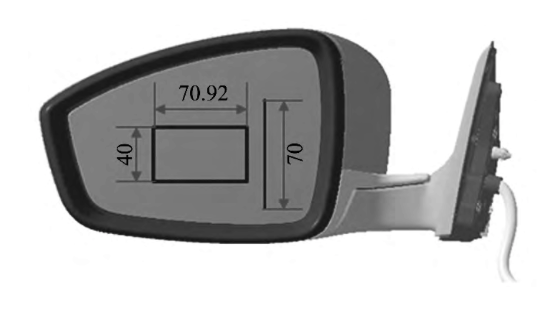
\includegraphics[width=12cm]{minsize.png}
\caption{国标中后视镜最小尺寸示意} \label{fig:后视镜最小尺寸示意}
\end{figure}

\par 放大后外后视镜镜片参数为:
$length = 72.48\times 2.72 = 197.1456$,            
$width = 70 \times 1.625 = 113.75$。(实际生产时切割出所需要的形状)

\subsubsection{平均畸变率的求解}

\par 通过方案一、方案二模型得到待定系数的镜面。以第一种方案为例:
\par 曲率半径较小的球面从$y$轴正方向看落在$XOZ$平面上的半径rr:

\begin{equation}
	\mathop{rr} = length \times \frac{cutRatio}{2}
\end{equation}

\par 外后视镜镜面上点的$y$坐标$f$:
\begin{equation}
	f = 
	\begin{cases}
		\sqrt{R_1^2 - (x-x_1)^2 - (z - z_1)^2} + y_1\quad \quad otherwise
		\\
		\sqrt{R_2^2 - (x-x_2)^2 - (z - z_2)^2} + y_2 \quad \quad 
		\sqrt{(x-x_2)^2 - (z - z_2)^2} < \mathop{rr} 
	\end{cases} 
\end{equation}

\par 将双眼中点坐标$(X_0,Y_0,Z_0)$作为求解平均畸变率所用的眼点坐标(单位mm):

\begin{equation}
	\begin{cases}
		X_0 = -450 \\ 
		Y_0 = 730 \\
		Z_0 = 0 
	\end{cases} 
\end{equation}




\par 已知曲面方程和曲面上一个固定点,通过公式(\ref{F})求得该点的切平面方程(公式(\ref{qiepingmian}))、法线方程(公式(\ref{faxian}))、法向量(公式(\ref{faxiangliang}))。
\begin{equation}
\label{F}
	\begin{cases}
		F_1 = f_x = diff(f,x) \\
		F_2 = f_z = diff(f,z) \\
		F_3 = f_y = -1
	\end{cases}
\end{equation}

\begin{equation}
\label{qiepingmian}
	(x - x_0)F_1(x_0,y_0,z_0) + (y - y_0)F_2(x_0,y_0,z_0) + (z - z_0)F_3(x_0,y_0,z_0) = 0
\end{equation}

\begin{equation}
\label{faxian}
	\frac{x - x_0}{F_1(x_0,y_0,z_0)} = \frac{y - y_0}{F_2(x_0,y_0,z_0)} = \frac{z - z_0}{F_3(x_0,y_0,z_0)} 
\end{equation}

\begin{equation}
\label{faxiangliang}
	\vec{n_0} = \left[\frac{F_1}{\sqrt{F_1^2+F_2^2+F_3^2}},\quad \frac{F_2}{\sqrt{F_1^2+F_2^2+F_3^2}},\quad \frac{F_3}{\sqrt{F_1^2+F_2^2+F_3^2}}\right]
\end{equation}
\par 给定入射光线方向向量$\vec{a}$:
\begin{equation}
	\vec{a} = [x - X_0,\quad f - Y_0, \quad z - Z_0 ]
\end{equation}
\par 通过公式(\ref{guiyi})将归一化,代入公式(\ref{b})中求得反射光线与光屏的交点坐标$(X_x,Y_y,Z_z)$(如公示(\ref{jiaodian})所示,其中dis为光屏与外后视镜的距离)。
\begin{equation}
\label{guiyi}
	\vec{a} = \frac{\vec{a}}{\|\vec{a}\|}   
\end{equation}

\begin{equation}
\label{b}
	\vec{b} = \vec{a} - 2 \cdot (\vec{a} \cdot \vec{n_0}) \cdot \vec{n_0}
\end{equation}

\begin{equation}
\label{jiaodian}
	\begin{cases}
		X_x = \frac{Y_y - Y}{b_y \cdot b_x} + X \\
		Y_y = dis \\
		Z_z = \frac{Y_y - Y}{b_y \cdot b_x} + Z
	\end{cases}
\end{equation}

\par 将外后视镜镜面以及光屏上对应点的数据代入公式(\ref{畸变率})中求解得到外后视镜的平均畸变率$\alpha$。

\subsubsection{视野范围的求解}
\begin{enumerate}
	\item 按照畸变率计算中的方法在外后视镜面上完成$50\times50$的投点。
	\item 与求畸变率不同,视野求解需要考虑左右眼的差距,此时眼点位置依据国家标准,在畸变率计算中确定的驾驶员坐标的基础上,水平增减$32.5mm$作为左右眼点的坐标。
	\item 对于水平视野范围计算,左后视镜:将屏放在10m的位置,分别计算左右眼水平视野最大宽度,综合取最大值。右后视镜时:将屏放在20m的位置,分别计算左右眼水平视野最大宽度,综合取最大值。
	\item 对于垂直视野范围计算,将光屏放置在汽车后轴的位置(按照常见量产车平均轴距确定),测量垂直方向上的最大视野范围。
	\item 剩下步骤与计算平均畸变率一致。
\end{enumerate}

\subsubsection{综合求解结果}
通过上述方法进行求解后得到如下表(\ref{计算结果1})所示的最终结果(单位为mm),对比方案一与方案二的结果,我们优先选择了方案一。
\begin{table}[!htbp]
\centering
\caption{外后视镜镜面方案计算结果}
\label{计算结果1}
\begin{tabular}{ccccccc}
\toprule
方法类别 & cutRatio & $R_2$ & $\alpha$ & $L$ & $H$ & $K$\\ \midrule

方案一左侧 &0.5 &    1100   &     3.82      \%    &4336  &   638 &  4170.37 \\
方案一右侧 & 0.2 &   1100    &     11.44\%   &11536       &966  &10216.8    \\
方案二左侧 &0.2 &    1100     &    3.97\% & 8696 & 600   & 8350.77\\                                                  
方案二右侧 & 0.2    & 1100      &   11.44\%           & 11536   & 966   & 10216.28  \\       
\bottomrule 
\end{tabular}
\end{table}

\par 如图(\ref{fig:DD1Z})所示为最终方案左侧外后视镜在10米处可观察到的视野范围(后视镜中线以上)。如图(\ref{fig:DD1Y})所示为最终方案右侧外后视镜在20米处可观察到的视野范围(后视镜中线以上)。


\begin{figure}[!htbp]  
\begin{minipage}[t]{0.5\textwidth}
\centering  
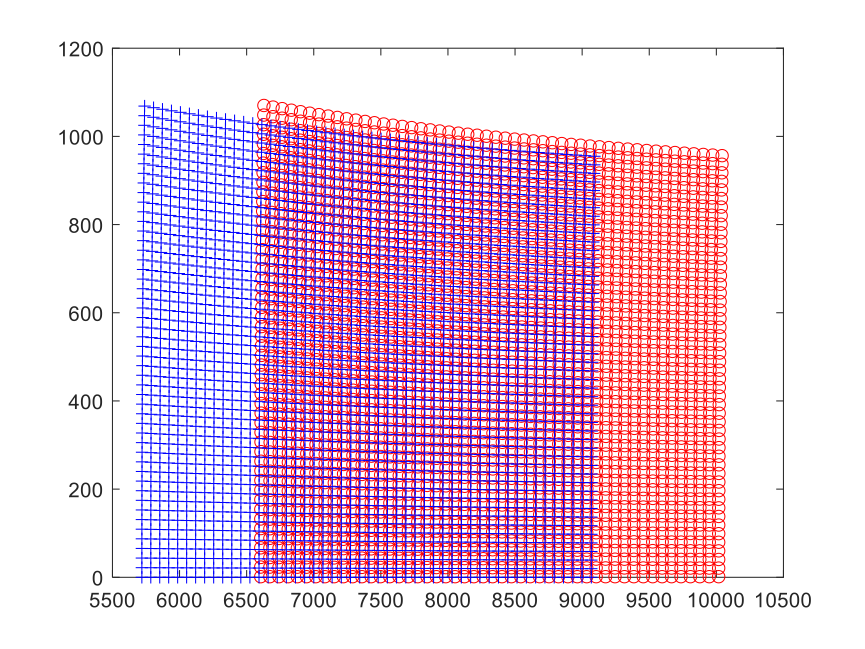
\includegraphics[width=\linewidth]{plan2-z.png}
\caption{左侧后视镜中线以上视野范围与图像畸变} \label{fig:DD1Z}\end{minipage}
\hspace{1ex}
\begin{minipage}[t]{0.5\textwidth}  
\centering  
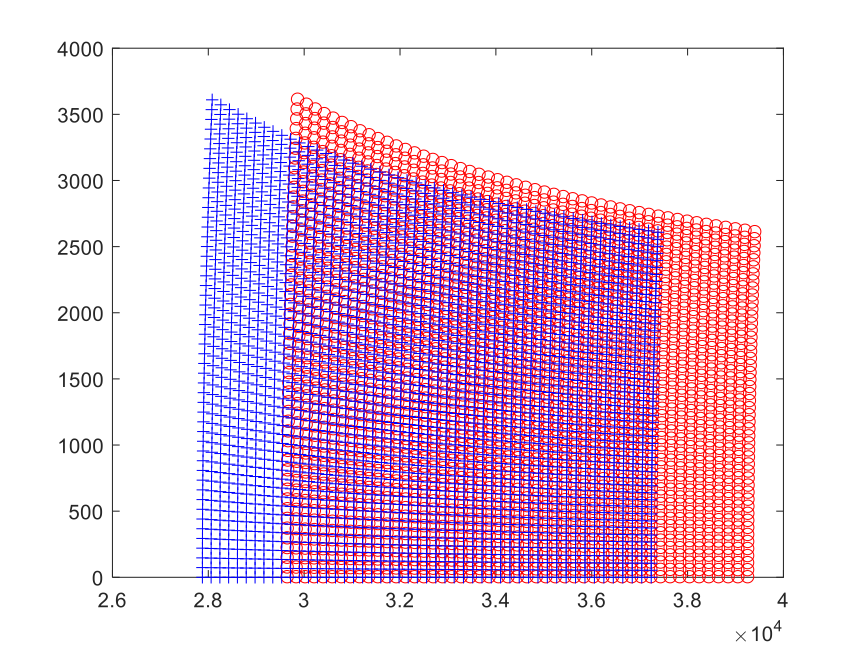
\includegraphics[width=\linewidth]{plan2-y.png}
\caption{右侧后视镜中线以上视野范围与图像畸变} \label{fig:DD1Y}\end{minipage}  
\end{figure} 

 
\subsubsection{外后视镜角度调整}
\par 由后视镜安装的初始位置一般难以符合视野的要求,所以必须将其调整到合适位置,使其视野能涵盖国标规定的区域。因此在安装时能对外后视镜片进行绕坐标轴的旋转。

\par 通过调整外后视镜的安装角度,可使得外后视镜视野范围覆盖国标要求的区域以及汽车后轮等区域。
 
\subsection{问题二求解}
\subsubsection{求解方法}

\par 本文以左外后视镜为例,给出一个简单的判断方法。通过查询资料,得到量产车辆的一般宽度(车身外侧钣金最突点之间的距离)为$W=1700mm$,因此首先将后车车头抽象为一条平均长度在1700mm的线段$c_1$,反射到后视镜上为线段$c_2$。左外后视镜分界线以左曲率半径小,畸变较大,只用来判断后方物体的有无,不用作距离远近和方位的判断。因而在$c_2$上选取如图(\ref{q2-1})所示的两个特征:$c_2$右端点距后视镜最右侧的距离和$c_2$长度占分界线以右长度$a$的比例。右后视镜同理如图(\ref{q2-2})所示。



\begin{figure}[!htbp]  
\begin{minipage}[t]{0.5\textwidth}
\centering  
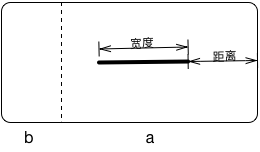
\includegraphics[width=\linewidth]{q2-z.png} \\
\caption{左后视镜} \label{q2-1}
\end{minipage}
\hspace{1ex}
\begin{minipage}[t]{0.5\textwidth}  
\centering  
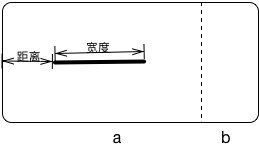
\includegraphics[width=\linewidth]{q2-y.png}\\
\caption{右后视镜}  \label{q2-2}
\end{minipage}  
\end{figure} 

\par 以本车左侧为例,如图(\ref{q2-3})所示定义纵向、横向车距。

\begin{figure}[!htbp]
\small
\centering
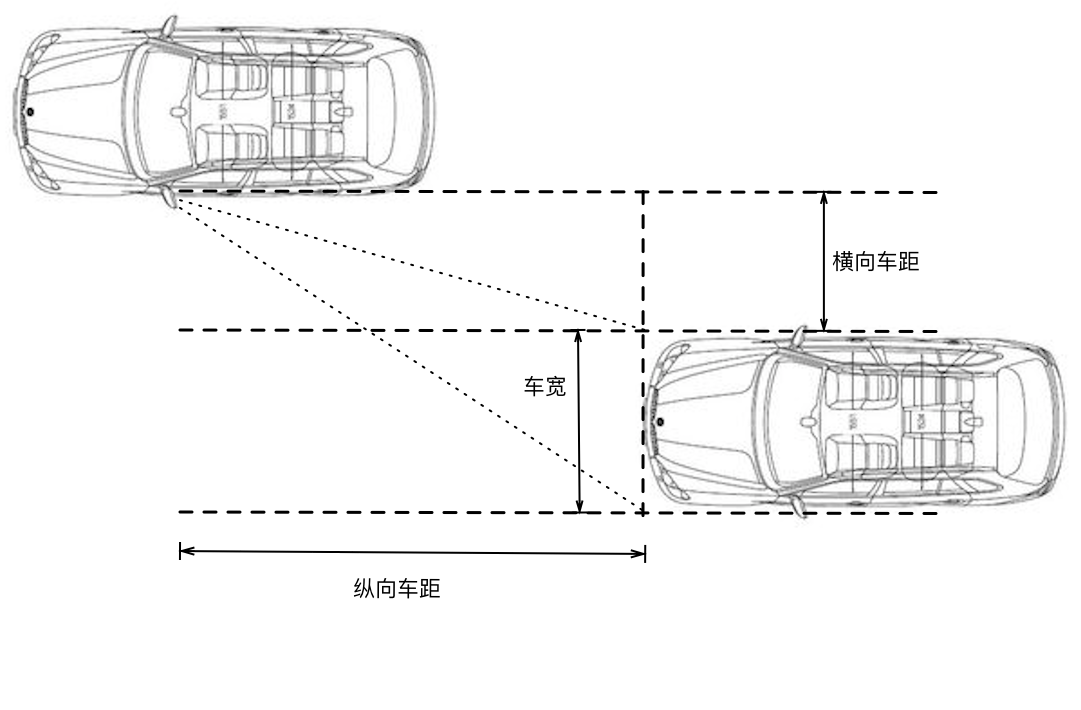
\includegraphics[width=14cm]{q2-3.png}
\caption{车距定义示意图} \label{q2-3}
\end{figure}

\par 本文通过多项式回归找到拟合的表达式,并用剩余标准差\upcite{剩余标准差}(如公式(\ref{剩余标准差公式})所示)来衡量误差。

\begin{equation}
\label{剩余标准差公式}
	S = \sqrt{\frac{Q}{f_Q}} = \sqrt{\frac{\sum\limits_{i = 1}^{n} \left( y_i - \hat{y_i} \right)^2}{n-2}}
\end{equation}

\subsubsection{综合求解}

\par 根据计算机模拟得出纵向车距(左外后视镜距后车车头的距离)和横向车距,结果如表(\ref{车距计算结果})所示。



\begin{table}[!h]
\centering
\caption{车距计算结果}
\label{车距计算结果}
    \begin{tabular}{|c|c|c|c|c|}
    \hline
    距右边距离占比                        & 占a区比例                        & 纵向车距(m) & 横向车距(m) & 观测到车宽(mm) \\ \hline
    $\frac{0}{5}$ & $\frac{1}{4}$ & 25   & 1    & 1720  \\ \hline
    $\frac{0}{5}$ & $\frac{1}{3}$ & 18   & 1    & 1667  \\ \hline
    $\frac{0}{5}$ & $\frac{1}{2}$ & 12   & 1    & 1696  \\ \hline
    $\frac{1}{5}$ & $\frac{1}{4}$ & 24   & 2   & 1676  \\ \hline
    $\frac{1}{5}$ & $\frac{1}{3}$ & 18   & 1    & 1689  \\ \hline
    $\frac{1}{5}$ & $\frac{1}{2}$ & 12   & 1    & 1716  \\ \hline
    $\frac{2}{5}$ & $\frac{1}{4}$ & 24   & 2    & 1695  \\ \hline
    $\frac{2}{5}$ & $\frac{1}{3}$ & 18   & 2    & 1707  \\ \hline
    $\frac{2}{5}$ & $\frac{1}{2}$ & 12   & 2    & 1731  \\ \hline
    $\frac{3}{5}$ & $\frac{1}{4}$ & 24   & 4    & 1709  \\ \hline
   	$\frac{3}{5}$ & $\frac{1}{3}$ & 17   & 3    & 1626  \\ \hline
    \end{tabular}
\end{table}

\par 通过表(\ref{车距计算结果})发现,$c_2$右端点距后视镜最右侧的距离对于纵向距离的估计影响很小,均在1米以内,因而忽略其影响,只考虑占a区比例对纵向距离的影响。取端点距右边距离为0时,细化$c_2$长度占a区长度的比例,计算得到表(\ref{车距细分计算结果})所示的结果。
\begin{table}[!h]
\centering
\caption{车距细分计算结果}
\label{车距细分计算结果}
    \begin{tabular}{|c|c|c|c|c|}
    \hline
  	占a区比例  & 纵向车距(m)  & 观测到车宽(mm) \\ \hline	
	$\frac{1}{5}$ & 31       	& 1697  \\ \hline
	$\frac{1}{4}$ & 25       	& 1720  \\ \hline
	$\frac{1}{3}$ & 18       	& 1667 \\ \hline
	$\frac{1}{2}$ & 12      	& 1696  \\ \hline
	$\frac{2}{3}$ & 9      	& 1723  \\ \hline
	$\frac{3}{4}$ & 8      	& 1736  \\ \hline
	$\frac{4}{5}$ & 7      	& 1637 \\ \hline
	1             & 6      	& 1773  \\ \hline
    \end{tabular}
\end{table}

\par 通过一元多项式拟合得到汽车在外后视镜a视野区中像的占比($x$)与后方汽车与本车后视镜间的距离($y$)关系如公式(\ref{q2-e-1})所示,其回归曲线如图(\ref{q2-huigui})所示,计算得到剩余标准差为4.0739。

\begin{equation}
\label{q2-e-1}
	y = 51.2573x^2 - 88.6317x + 44.4255
\end{equation}


\begin{figure}[h]
\small
\centering
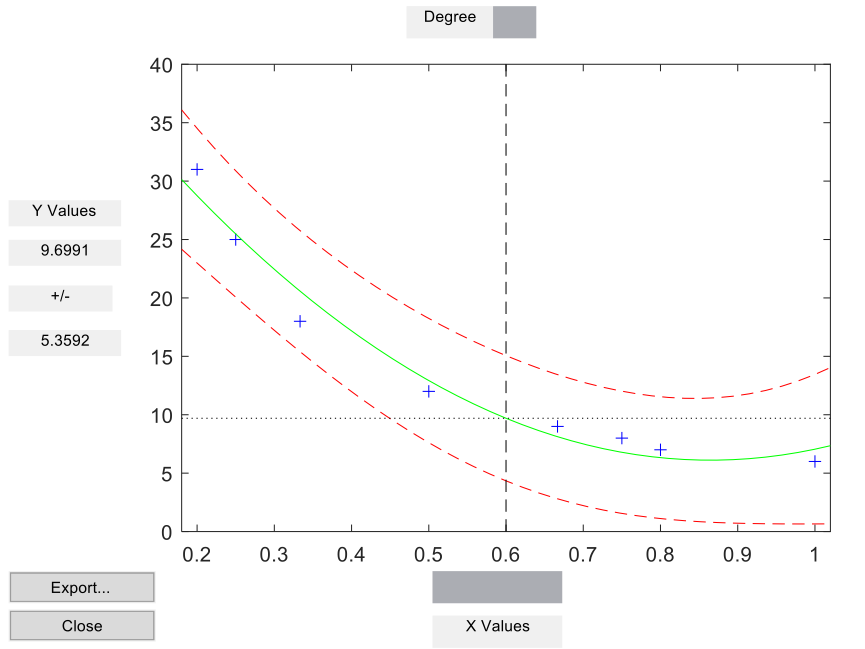
\includegraphics[width=12cm]{q2-huigui.png}
\caption{汽纵向距离拟合曲线} \label{q2-huigui}
\end{figure}



\par 在求解水平距离时,需综合考虑距右边距离和占a区比例的影响,本文采用多元二项式回归进行拟合,得到汽车的像的右边缘距a区右侧的距离($x_1$)、 在外后视镜a视野区中占比($x_2$)与后方汽车与本车后视镜间的距离($y$)关系如公式(\ref{q2-e-1})所示,其回归曲线如图(\ref{q2-huigui-shuiping})所示,计算得到剩余标准差为0.3265。

\begin{equation}
	y = 4.976 - 0.1344 x_1 -21.0161 x_2 - 6.8548 x_1^2 + 25.7419 x_2^2
\end{equation}



\begin{figure}[h]
\small
\centering
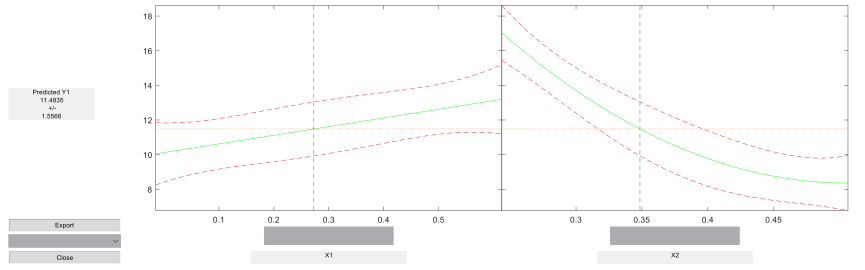
\includegraphics[width=12cm]{q2-huigui-shuiping.png}
\caption{汽车横向距离拟合曲线} \label{q2-huigui-shuiping}
\end{figure}


\par 驾驶员可按照上表(\ref{车距计算结果})通过后车的像在左外后视镜a区中宽度的占比大致确定后车纵向距离,通过后车的像的右边缘距左外后视镜右边缘的距离占比确定后车横向距离。


\subsection{问题三求解}
\par 在问题三中,我们选取量产车:奇瑞QQ 2013款(如图(\ref{fig:qq3})所示),通过本文建立的模型测算其外后视镜视野范围、图像畸变率等参数。该车原外后视镜尺寸为$165mm \times 126mm$ 曲率半径为$1200mm$。
\begin{figure}[h]
\small
\centering
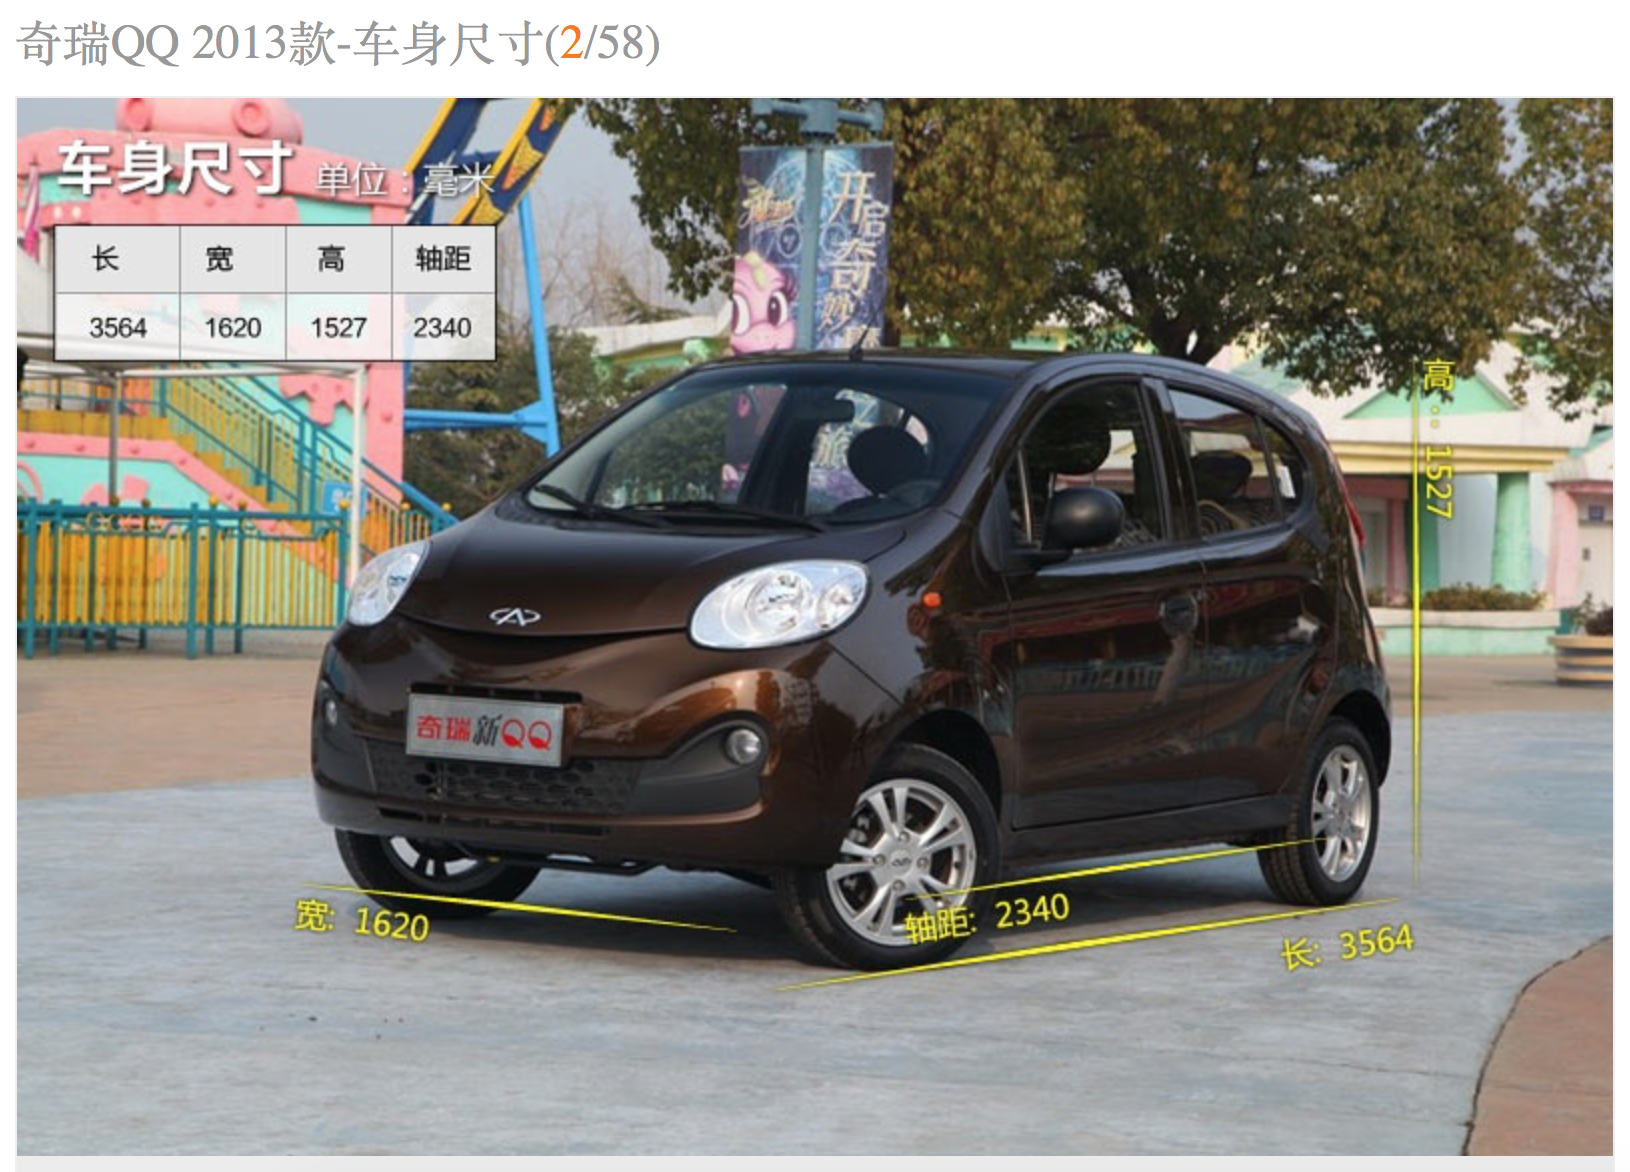
\includegraphics[width=12cm]{qq3.png}
\caption{奇瑞QQ 2013款外形尺寸图} \label{fig:qq3}
\end{figure}

计算得原后视镜相关参数如下表(\ref{原车后视镜计算数据})所示:
\begin{table}[!htbp]
\centering
\caption{原车后视镜计算数据}
\label{原车后视镜计算数据}
\begin{tabular}{|c|c|c|}
\toprule
左后视镜视野范围(mm)$L$ & 左后视镜畸变率$\alpha$ & 左后视综合指标$K$ \\ \hline 
4553.20823986563 & 2.88920268960021\%  & 4421.65682493633 \\ \hline 


右后视镜视野范围(mm)$L$ & 右后视镜畸变率$\alpha$  & 右后视综合指标$K$ \\ \hline
7997.14730406906 & 10.2758921450585\%  &  7175.36907242147 \\

\bottomrule 
\end{tabular}

\end{table}
\par 如图(\ref{fig:qiruiz},\ref{fig:qiruiy})所示分别为原车后视镜的外后视镜中线以上视野范围。


\begin{figure}[!htbp]  
\begin{minipage}[t]{0.5\textwidth}
\centering  
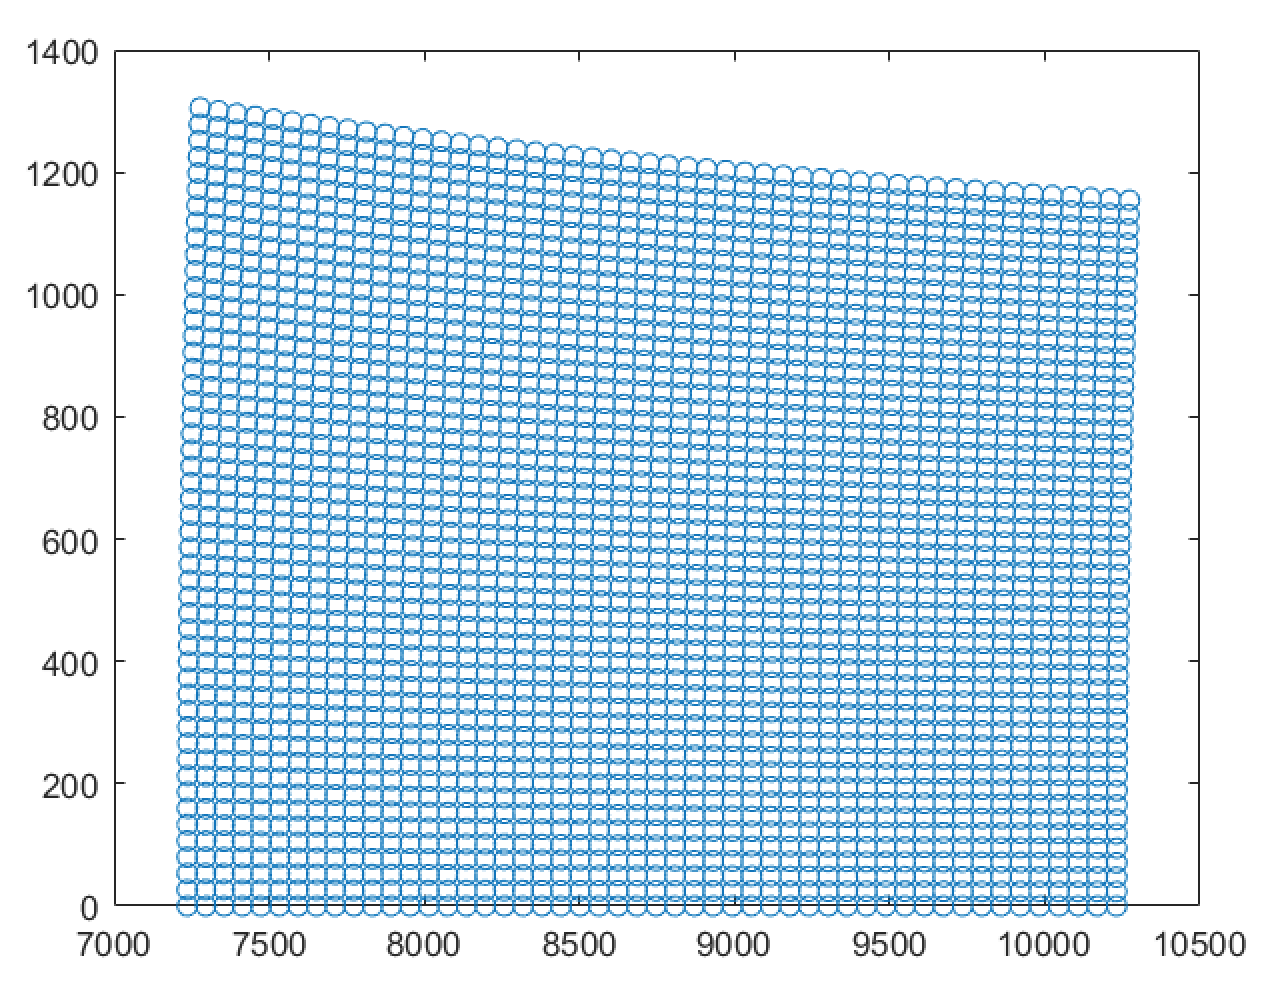
\includegraphics[width=\linewidth]{qiruiz.png}
\caption{原车左侧后视镜视野范围(中线以上)} \label{fig:qiruiz}\end{minipage}
\hspace{1ex}
\begin{minipage}[t]{0.5\textwidth}  
\centering  
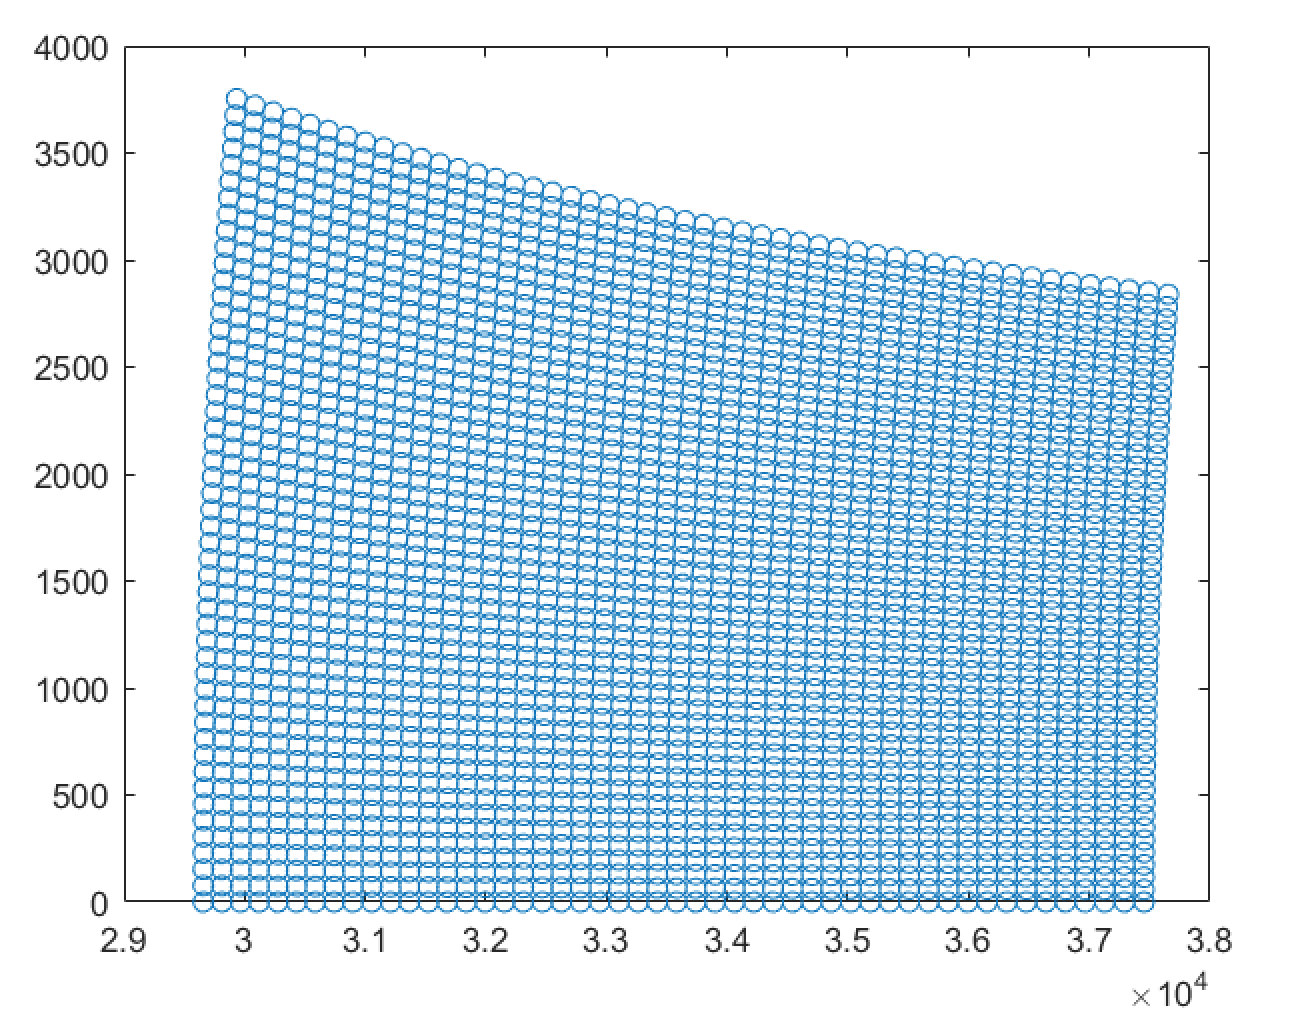
\includegraphics[width=\linewidth]{qiruiyou.png}
\caption{原车右侧后视镜视野范围(中线以上)} \label{fig:qiruiy}
\end{minipage}  
\end{figure} 

 
\par 同时我们设计的双曲率后视镜采取曲率半径分别为$1260mm$与$500mm$,得到驾驶员的左侧视野范围为$5527mm$,畸变率为$3.8\%$;右侧的视野范围为$11536 mm$,畸变率为$11.4\%$。

\par 本文设计的外后视镜模型在畸变率基本没变的基础上将左右两侧的视野范围大大增加,因此我们的设计更优于原车设计。


\section{模型优缺点}
\subsection{模型优点}
\begin{enumerate}
	\item 畸变率模型创新性地提出了凸面镜图像畸变率的定量化刻画方法,并且该指标经检验是合理的。
	\item 双曲率外后视镜是市场上最流行的设计,并且本文设计的双曲率外后视镜,很好的符合了国家标准,并尽可能在保证失真率可控的前提下提高了后视镜视野范围。
	\item 双曲率外后视镜设计是依据车型、驾驶员眼点位置与后视镜相对位置、视野要求三个要素,运用光学原理和计算机模拟方法,对车辆的左右不同视野角度选择不同的曲率半径。在失真率可接受的条件下实现扩大视野、减少盲区的目的。
\end{enumerate}
\subsection{模型缺点}
\begin{enumerate}
	\item 外后视镜模型没有考虑双曲率球面在拼接过程中的边缘的平滑过渡问题。
	\item 在畸变率模型中,算法的复杂度高,计算耗时长。
\end{enumerate}
\section{模型改进方向}
\begin{enumerate}
	\item 在构造外后视镜模型的时候,选取不同的曲率半径的两种球面拼接而成,在改进工作中,需要考虑用一般的二次曲面来构造外后视镜。该方法能构造出变曲率外后视镜,并且不需要考虑镜面区域的过渡区域的问题。
	\item 本文设计的畸变率的计算模型,复杂度比较高,在计算机求解过程中,运算时间比较长,在改进过程中建立实际图像与后视镜反射后的图像的重叠程度作为畸变率模型的新指标。
\end{enumerate}


%参考文献
\begin{thebibliography}{9}%宽度9
 \bibitem{大视野后视镜} 王卫华. 汽车大视野后视镜的理论建模与应用技术研究[D]. 武汉理工大学, 2006.
 \bibitem{后视镜设计} 周博. 汽车外后视镜镜片尺寸及位置设计[J]. 上海汽车, 2015(12):41-44.
 \bibitem{后视镜仿真} 牛慧超. 汽车后视镜检测系统的研究及仿真设计[D]. 武汉理工大学, 2009.
 \bibitem{GB} GB 15084-94 汽车后视镜的性能和安装要求
 \bibitem{汽车分类}\url{https://www.zybang.com/question/cf0e112815df2cd96348c0e973e0a546.html}
 \bibitem{剩余标准差} \url{http://baike.baidu.com/link?url=ZHnyqmzYJbm6QayDkOHQ5ZmM-4Yq4bbgRDUFllJ_nk7wS4lpTxxFKuHKCr2cr9MeuENIsMVkLY3L3y5gn57eDarr51Pklm1RArkCHendwbcWYB3POIVxcQwYsNxeP6nMbWQrYYoI9iH2oceYnzfxLK}
 
\end{thebibliography}

\newpage
%附录
\appendix

\section{附件内容}
\begin{enumerate}
	\item 计算中间数据.xlsx
	\item 程序.zip
\end{enumerate}



\end{document} 